%!TeX root = application
\documentclass[../main.tex]{subfiles}

\begin{document}
    \section{Gate driver's transient response} \label{sec:result_gate_driver}
    \justify
    The followings are voltage traces of the drain voltage (green) and the gate (yellow) voltage of the MOSFET during a turn-off event.

    \begin{figure}[!h]
        \centerline{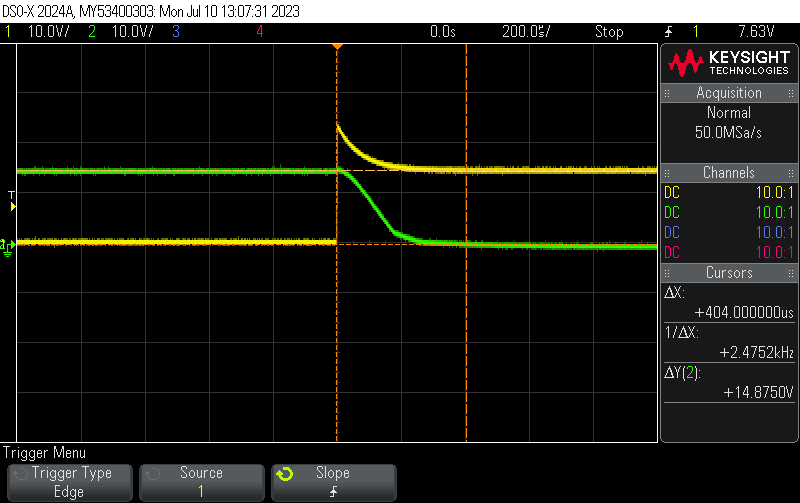
\includegraphics[scale=0.5]{media/turn_off_no_load.png}}
        \caption{MOSFET's source and gate voltage during turn off without load.}
        \label{fig:turn_off_no_load}
    \end{figure}

    \begin{figure}[!h]
        \centerline{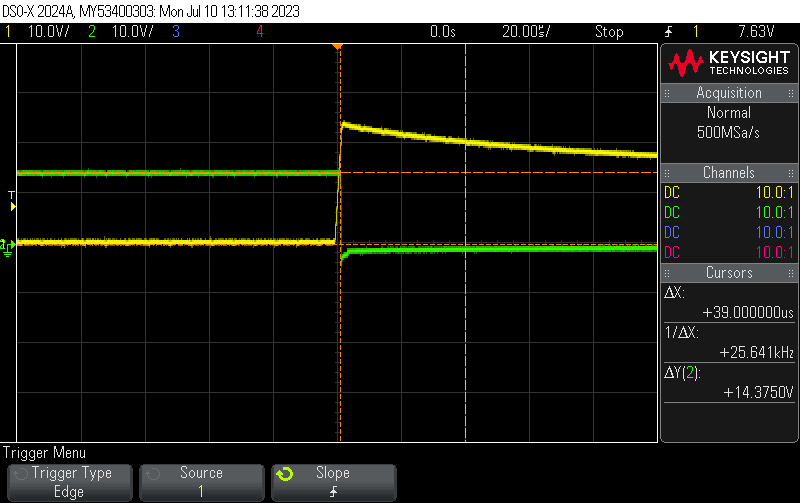
\includegraphics[scale=0.5]{media/turn_off_4_7_load.png}}
        \caption{MOSFET's source and gate voltage during turn with $4.7\Omega$ load.}
        \label{fig:turn_off_4_7_load}
    \end{figure}

    \pagebreak
    \justify
    The peak in the gate voltage is a result of the MOSFET switching transient response. For a P-channel MOSFET, a turn-off event results in gate capacitance discharge. Similar to equation \eqref{eq:gate_charge_til_miller}, $V_{gs, miller}$ for a P-channel MOSFET can be calculated:

    \begin{equation}
        V_{gs, miller} = V_{signal}\left[\exp{\left(-\dfrac{\Delta t_{0\rightarrow2}}{R_{g}(C_{gs} +C_{gd})}\right)}\right]
    \end{equation}

    \justify
    The following observations can be made:
    \begin{itemize}
        \item In the datasheet of IRF4905S, $C_{gs} +C_{gd} = C_{iss}(V_{ds}) = 1448pF$. 
        \item The source terminal of the MOSFET is always connected to the input supply votlage, therefore, $V_{gs, miller}=V_{g, miller} - 15V$.
        \item In the proposed gate driver topoloy, the gate is pull-up to supply voltage, thus, $V_{signal} = V_{in} = 15V$.
    \end{itemize}
    \justify
    Then, the above equation becomes:
    
    \begin{equation}
    \begin{split}
        V_{g, miller} - 15V &= V_{signal}\left[\exp{\left(-\dfrac{\Delta t_{0\rightarrow2}}{100k\Omega\cdot 1448pF}\right)}\right] \\
        \Leftrightarrow V_{g, miller} &= V_{signal}\left[\exp{\left(-\Delta t_{0\rightarrow2}\cdot 6900 s^{-1}\right)}\right] + 15V \geq 15V \text{for all } Delta t_{0\rightarrow2}       
    \end{split}
    \end{equation}

    \justify
    Let:
    \begin{equation}
    \begin{split}
        \Delta t_{0\rightarrow2} &\in [100\mu s;200\mu s] \\
        \Leftrightarrow V_{g, miller} &\in [1.25V_{in}; 1.5V_{in}] = [18.75V; 22.5V]
    \end{split}
    \end{equation}

    \justify
    The above range for $V_{g, miller}$ agrees with the measured response. Thus, the desired effect of quick turn-off for the gate driver can only be achieved with a snubber circuit whose design steps are thoroughly documented by chip makers \cite{RohmSnubber} \cite{InfineonSnubber}. The general principle of a snubber is limiting the $dv/dt$ of voltages across the Drain-Source region at device turn-off. 

    \justify
    However, considering the the load is pure resistive, the $V_{g, miller}$ spike does not affet the load. In future development, this needs to be investigated to limit long-term damage to the MOSFETs, and to use for other types of load (inductive and/or capacitive).

    \pagebreak
    \section{Power-rail's component failure} \label{sec:result_power_rail}

    \subsection{LM2596}
    \justify
    The LM2596 IC chosen for the final PCB product was not sourced from trusted vendor, resulting in fluctuating $V_{ref\_LM2596}$ whose range is $[1.0V;1.23V]$. In the official datasheet \cite{LM2596}, the documented value of $V_{ref\_LM2596}$  is $1.23V$. This results in inaccurate output voltage $V_{out, sw}$ leading to higher $P_{loss}$ in creating the $5V$ rail. However, $V_{out, sw}$ is within the rated input voltage of the linear voltage regulator L7805. Thus, the operation of the 5V rail and other related subcircuits (latch, overvoltage detection subcircuit, and INA226) are guaranteed.

    \subsection{B0505S-2WR2}
    \justify
    The output voltage drops to below $3V$ when load (MCU) is attached. This is due to the input voltage tolerance not within the documented value of $\pm 10\%$. When at full capacity, the output of L7805 fluctuates within $[4.9V; 5V]$; and when at $4.9V$, the B0505S-2WR2 fails to outputs $5V$. The following solutions have been attempted:

    \begin{itemize}
        \item Maintain the minimum load requirement of $20\%$ of the B0505S-2WR2 by paralleling a resistor.
        \item Adjust input and output decouple capacitors.
    \end{itemize}

    \justify
    Thus, in the final product, the MCU is powered by an external $5V$ source via USB. This effectively makes the final product less portable.

    \pagebreak
    \section{Latch and protection subcircuits' performance} \label{sec:result_latch_circuit}.
    \justify
    \begin{itemize}
        \item All protection signal sources (overvoltage, undervoltage, overcurrent, and over-power) detects the set threshold, and their outputs are able to drive the latch subcircuit.
        \item The single op-amp latch subcircuit is able to received positive pulses as inputs, and outputs digital signal for the gate driver.
        \item Overlapping occurence of both turn-on and turn-off signals was not accounted for. Consider the case where a turn-on signal would result in overcurrent:
        \begin{itemize}
            \item The user presses the manual on button, and, immediately, a turn-off signal will be sent. 
            \item If the button is kept pressed, there will be a on-off oscillation at the output.
        \end{itemize}
        This behaviour is not desirable, and, instead, it should be notified when the user tries to close the switch after a fault is detected. The following figure shows a possible implementation of such behaviour. Because over-power and overvoltage detection are done by other component, their fault must be sent to the MCU, requiring an addition digital isolator.

        \begin{figure}[!h]
            \centerline{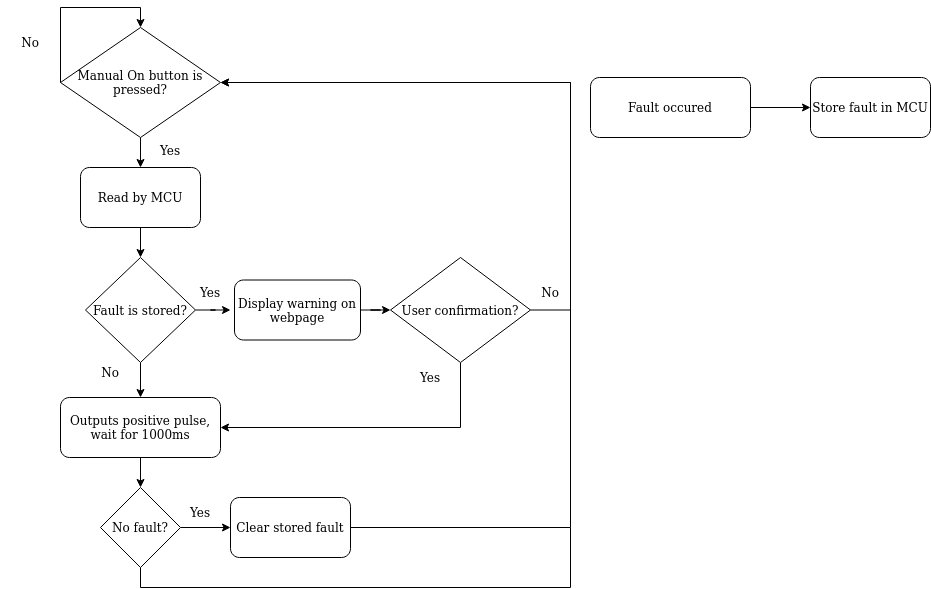
\includegraphics[scale=0.5]{media/turn_on_warning.drawio.png}}
            \caption{Possible implementation for closing the switch after a fault occurence.}
            \label{fig:turn_on_warning}
        \end{figure}

    \end{itemize}

    \pagebreak
    \section{Firmware and Application} \label{sec:result_fw_app}.
    \justify
    The MCU and the server hosted on a client's PC is able to perform well. By using the UDP protocol and sending the packet to 255.255.255.255, the MCU saves resources on waiting for response (in case of HTTP or TCP), and checking whether the host is alive to send. Furthermore, visualizing the data is non-critical which is suitable for UDP.

    \justify
    In previous implementation, the data is requested at the same rate of upload of the MCU - $10Hz$. However, the overhead of the function \lstinline{Plotly.extendTraces} increase the CPU usage at $10Hz$ update rate. Rather, the graph is updated at a lower rate, and with more data points, which reduces half of the CPU usage of Plotly.
\end{document}